\section{Results}\label{sec:results}

\paragraph*{Instrument} Every model returned a usable allocation for almost every prompt: refusals are at most \refusalMax\% and parse failures at most \failMax\% per model, so no model is excluded. Many replies miss 100 in arithmetic: the median model has \renormWideMedian\% of replies outside 95--105 after one retry, and one model \renormWideMax\% (Fig.~\ref{fig:rates}); these are renormalised under amendment~A1, and the original rule is a robustness check.

\paragraph*{Home tilt (H1)} Table~\ref{tab:primary} reports Eq.~\eqref{eq:main}. A model's home market receives $\beta=\betaHome{}$\,pp (SE \betaHomeSE{}; wild template bootstrap 95\% CI \betaWildLo{} to \betaWildHi{}) relative to what other models give that market. The estimate is small against an equal weight of 12.5\,pp and has the opposite sign to H1, which is \emph{not supported}. Per model (Fig.~\ref{fig:tilt}), the home tilt ranges from \tiltMin{} to \tiltMax{}\,pp: \nTiltPos{} models allocate significantly more to their home market than other models do and \nTiltNeg{} allocate significantly less, with no consistent pattern within origin groups. By group, Chinese models allocate \betaChina{}\,pp more to China, European models \betaEurope{}\,pp to the Eurozone, US models \betaUnitedstates{}\,pp to the United States, Thai models \betaThailand{}\,pp to Thailand and the Korean model \betaKorea{}\,pp to South Korea. Among English prompts with no investor nationality (H2), $\beta=\betaHtwo{}$\,pp (SE \betaHtwoSE{}; only 12 prompts), so H2 is not supported either.

\begin{figure}[t]
\centering
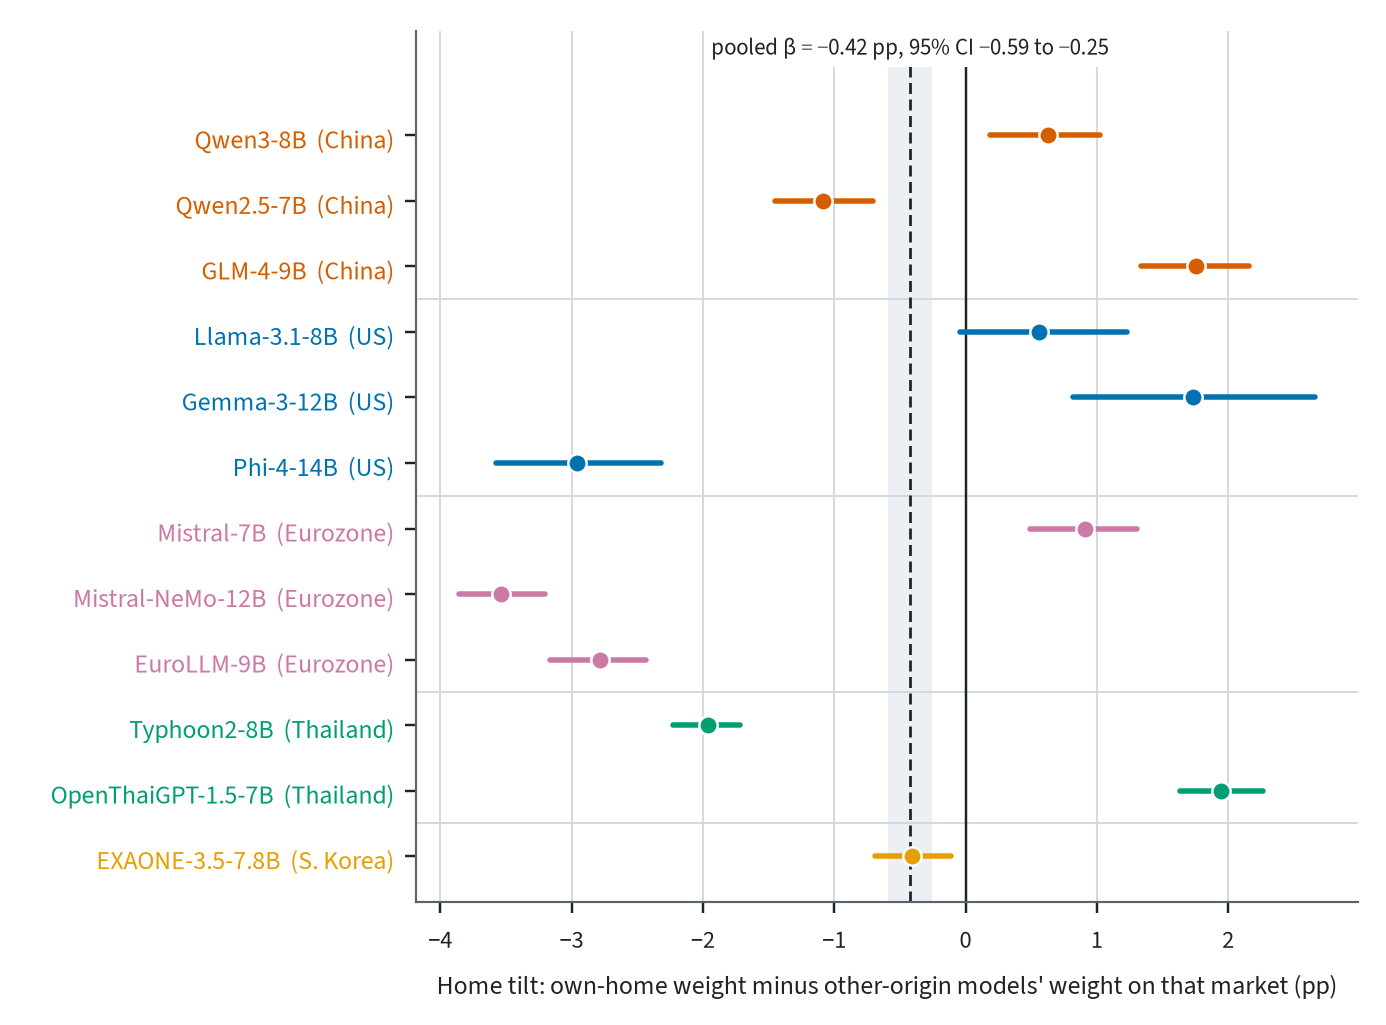
\includegraphics[width=\columnwidth]{figures/fig1_home_tilt.png}
\caption{Home tilt by model: mean weight on the model's home market minus the mean weight that models of other origins give that market on the same prompt, with 95\% prompt-bootstrap CIs.}
\label{fig:tilt}
\end{figure}

\paragraph*{Origin, investor and language} The prompt moves allocations more than the model's origin does. When the investor states a country of residence, that market receives $\gamma=\gammaInv{}$\,pp more (SE \gammaInvSE{}); writing the prompt in a market's main language adds $\lambda=\lambdaLang{}$\,pp (SE \lambdaLangSE{}; Fig.~\ref{fig:decomp}). Levels are far from both market-capitalisation and GDP weights (Fig.~\ref{fig:heatmap}): every model gives the United States \usShareMin--\usShareMax\% (MSCI ACWI, proxied by an ACWI-tracking ETF's holdings on 29~October 2026 and renormalised over the eight markets: \acwiUS\%) and China \chinaShareMin--\chinaShareMax\% (ACWI: \acwiChina\%), so all models sit much closer to equal weight than to any capitalisation benchmark.

\begin{figure*}[t]
\centering
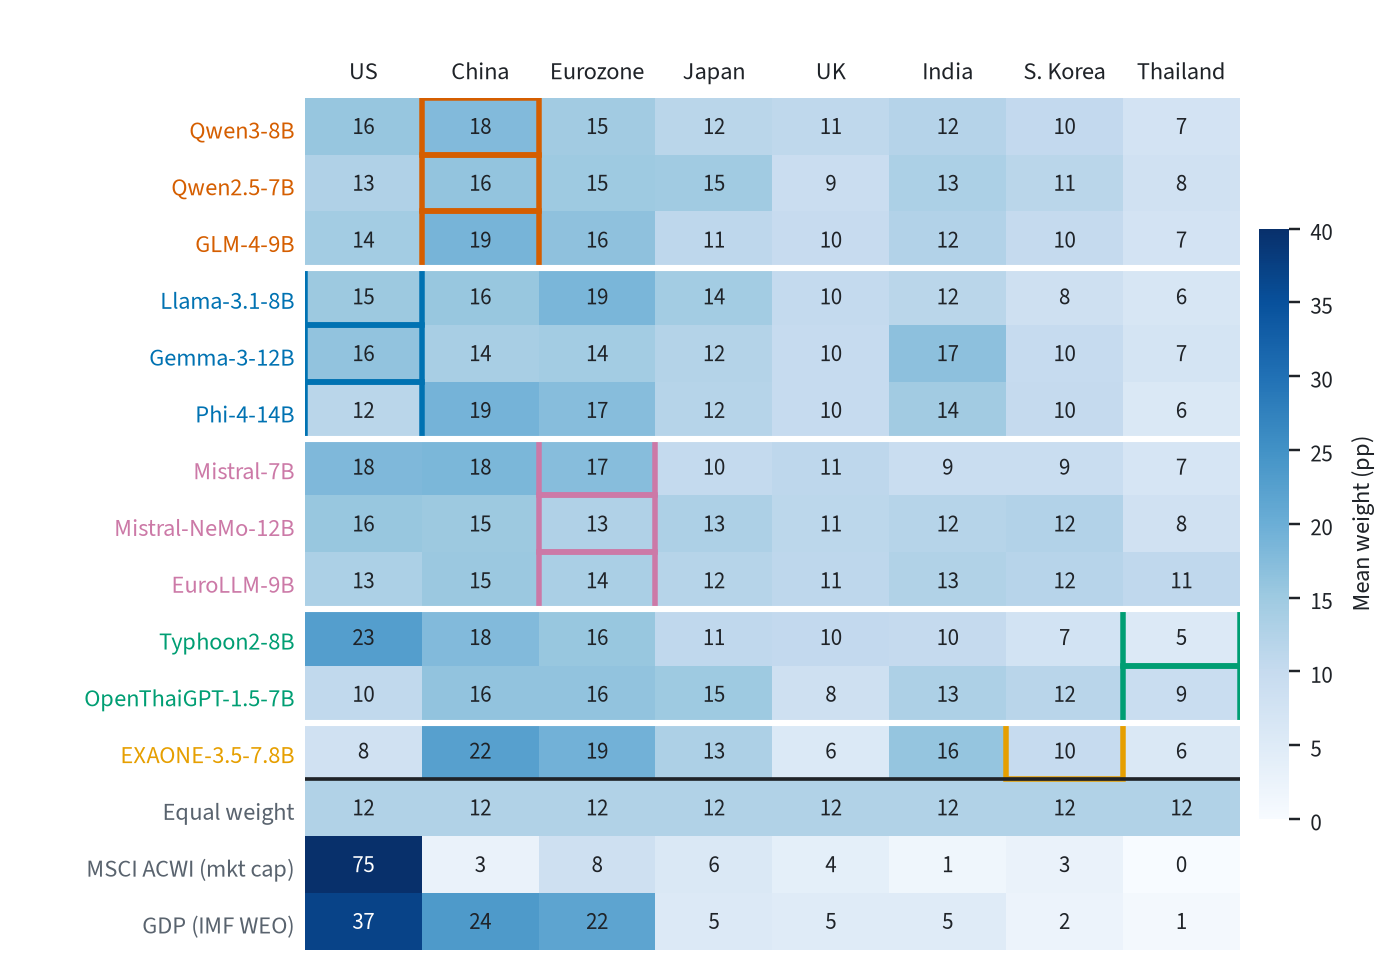
\includegraphics[width=0.49\textwidth]{figures/fig2_allocation_heatmap.png}\hfill
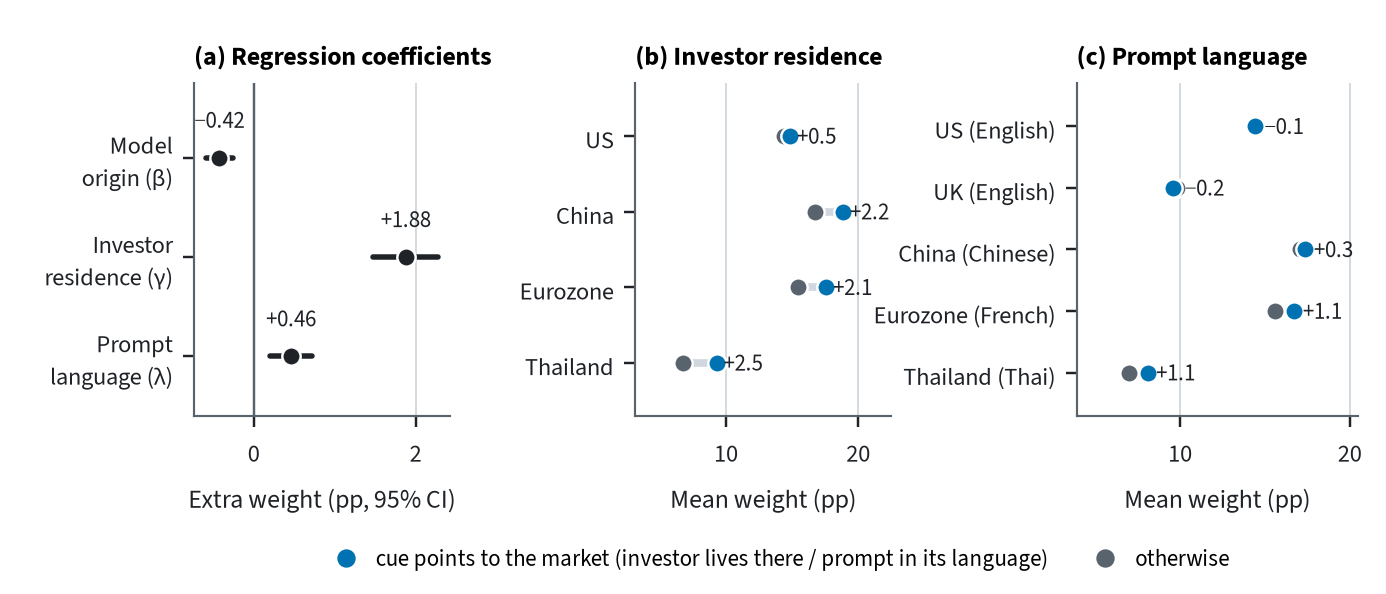
\includegraphics[width=0.49\textwidth]{figures/fig3_origin_vs_language_vs_investor.png}
\caption{Left: mean allocation by model and market (home cells outlined) with equal, market-capitalisation and GDP reference rows. Right: the three channels $\beta$, $\gamma$, $\lambda$ with 95\% CIs, and the China weight by prompt language and investor residence.}
\label{fig:heatmap}\label{fig:decomp}
\end{figure*}

\begin{table}[t]
\caption{Primary and secondary estimates (pp). SEs clustered by prompt.}
\label{tab:primary}
\centering
\begin{adjustbox}{max width=\columnwidth}
% generated by src/viz/paper_tex.py
\begin{tabular}{@{}lrrrrr@{}}
\toprule
 & Estimate (pp) & SE & $p$ & $N$ & Models \\
\midrule
\multicolumn{6}{@{}l}{\textit{Pooled regression, Eq.~\eqref{eq:main}; SE clustered by prompt}} \\
\quad $\beta$ Home (model origin) & \ensuremath{-}0.42 & 0.09 & $<$0.001 & 23,008 & 12 \\
\quad $\gamma$ InvestorHome & +1.88 & 0.21 & $<$0.001 & 23,008 & 12 \\
\quad $\lambda$ LanguageHome & +0.46 & 0.13 & 0.001 & 23,008 & 12 \\
\quad $\beta$ Home, wild cluster bootstrap over 8 templates (95\% CI) & \multicolumn{3}{r}{[\ensuremath{-}0.75, \ensuremath{-}0.09]} & 23,008 & 12 \\
\addlinespace
\multicolumn{6}{@{}l}{\textit{Home effect by origin group ($\beta \times$ group, same specification)}} \\
\quad Chinese models & +0.60 & 0.15 & $<$0.001 & 23,008 & 12 \\
\quad US models & \ensuremath{-}0.17 & 0.26 & 0.513 & 23,008 & 12 \\
\quad European models & \ensuremath{-}2.07 & 0.13 & $<$0.001 & 23,008 & 12 \\
\quad Thai models & +0.07 & 0.12 & 0.573 & 23,008 & 12 \\
\quad Korean model & \ensuremath{-}0.40 & 0.16 & 0.014 & 23,008 & 12 \\
\addlinespace
\multicolumn{6}{@{}l}{\textit{H2: English prompts with an unspecified investor}} \\
\quad $\beta$ Home & \ensuremath{-}1.02 & 0.29 & $<$0.001 & 1,152 & 12 \\
\addlinespace
\multicolumn{6}{@{}l}{\textit{H3: Thai fine-tune minus its base model, weight on Thailand (prompt fixed effects)}} \\
\quad $\delta$ Typhoon2-8B vs Llama-3.1-8B & \ensuremath{-}1.04 & 0.26 & $<$0.001 & 480 & 2 \\
\quad $\delta$ OpenThaiGPT-1.5-7B vs Qwen2.5-7B & +1.26 & 0.27 & $<$0.001 & 480 & 2 \\
\addlinespace
\multicolumn{6}{@{}l}{\textit{Cash currency: home currency chosen (linear probability model, pp)}} \\
\quad $\beta$ Home & \ensuremath{-}2.18 & 0.48 & $<$0.001 & 23,008 & 12 \\
\bottomrule
\end{tabular}

\end{adjustbox}
\end{table}

\paragraph*{Fine-tuning (H3)} The two Thai fine-tunes move in opposite directions (Fig.~\ref{fig:ft}). OpenThaiGPT allocates \ftOpenthaigptoneFiveSevenb{}\,pp more to Thailand than its base Qwen2.5-7B (\ftOpenthaigptoneFiveSevenbMean\% vs \ftOpenthaigptoneFiveSevenbBaseMean\%), whereas Typhoon2 allocates \ftTyphoontwoEightb{}\,pp relative to Llama-3.1-8B (\ftTyphoontwoEightbMean\% vs \ftTyphoontwoEightbBaseMean\%). H3 is supported for one pair only, so fine-tuning on Thai data is not associated with a consistent shift towards Thailand.

\begin{figure}[t]
\centering
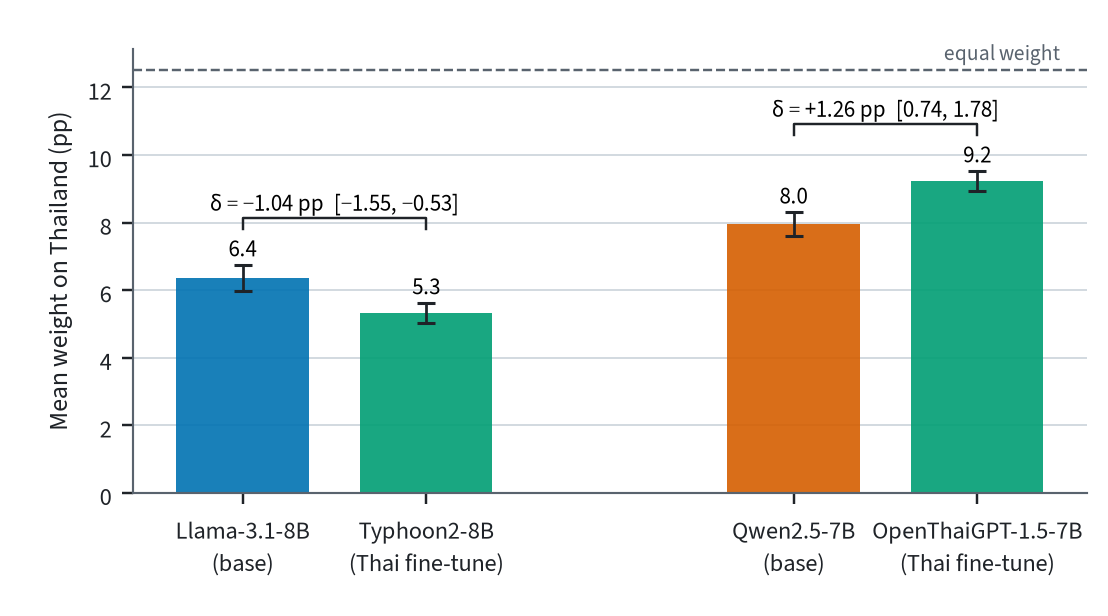
\includegraphics[width=\columnwidth]{figures/fig4_finetune_transmission.png}
\caption{Thailand weight of each Thai fine-tune and its base model, with 95\% CIs for the difference (prompt fixed effects).}
\label{fig:ft}
\end{figure}

\paragraph*{Cash currency} Every model chooses US dollars for cash in \usdCashMin--\usdCashMax\% of replies; the home-currency premium in the linear probability model is \cash{}\,pp (SE \cashSE{}). The high home-currency share of US models is the common dollar default, not a home effect.
